%!TEX root = ../masters_thesis.tex

\section{Editing Hivent Data} % (fold)
\label{sec:editing_hivent_data}

The previous section proposed the abstract Hivent Model, a set of Hivent operations and a visualization method. However, one purpose of the HGIS developed in this thesis is to add, alter and delete historical changes. This section presents the tools and methods to edit spatio-temporal data about the evolution of Areas in the Hivent Model. Whereas the Hivent Operations are well-defined and specific, user studies have shown that they are not well understood by humans to edit Areas. This thesis therefore introduces a different set of six \emph{Edit Operations} in section \ref{sub:edit_operations}. Afterwards, section \ref{sub:edit_workflow} shows a \emph{workflow} to perform an Edit Operation step by step. The Hivent Model needs to support editing historical changes in between other historical changes. The last section \ref{sub:retrospective_updates} explains the theoretical approach to \emph{retrospecitve updates} of spatio-temporal data in the Hivent Model.


% ------------------------------------------------------------------------------
\subsection{Edit Operations} % (fold)
\label{sub:edit_operations}

The Hivent Operations are valuable, because they can describe all possible changes in the evolution of Areas in time and space. They are really well understood from the system point of view and form the basis for the Hivent Model. However, one purpose of the HGIS developed in this thesis is to provide a well understood user interface to edit historical changes to Areas.

Throughout the development process, interviews with researchers in humanities at University of Virginia were conducted to understand their mental model about the task. It turned out that the Hivent Operations are not suitable to be used for human edit purposes, because of their low-level nature. One example is that the operations do not provide a straightforward way to create a new Area on previously unclaimed land. The same is true for changing the formal name of an Area. Therefore, this thesis introduces a second set of operations: five high-level \emph{Edit Operations} describe changes to countries on the map (see table \ref{tab:edit_operations}). They have proven to be understandable in several user studies.

\vspace{0.5em}
\begin{table}[H]
\begin{center}
\begin{tabular}{m{0.75cm} m{0.8cm} m{2.4cm} m{9.1cm}}
  \raisebox{-0.35\height}
  {
\includegraphics[width=0.72cm]{graphics/development/edit_operations/CRE}} &
  \texttt{CRE} & Create &
  a new Area with a new name and territory on the map. \\

  \raisebox{-0.35\height}
  {
\includegraphics[width=0.72cm]{graphics/development/edit_operations/MRG}} &
  \texttt{MRG} & Merge &
  two or more Areas to a new Area. The name has to be set manually, the territory is automatically unified. \\

  \raisebox{-0.35\height}
  {
\includegraphics[width=0.72cm]{graphics/development/edit_operations/DIS}} &
  \texttt{DIS} & Dissolve &
  one Area into two or more new Areas, manually setting their new territory and name. \\

  \raisebox{-0.35\height}
  {
\includegraphics[width=0.72cm]{graphics/development/edit_operations/CHB}} &
  \texttt{CHB} & Change Borders &
  between two neighboring Areas by defining the territory that changes sides. \\

  \raisebox{-0.35\height}
  {
\includegraphics[width=0.72cm]{graphics/development/edit_operations/REN}} &
  \texttt{REN} & Rename &
  an Area and set a new formal name, short name or both. \\

  \vspace{0.35em}
  \raisebox{-0.35\height}
  {
\includegraphics[width=0.72cm]{graphics/development/edit_operations/CES}} &
  \texttt{CES} & Cease &
  an Area by deleting it from the map, leaving unclaimed land. \\

\end{tabular}
\caption{The six Edit Operations}
\label{tab:edit_operations}
\end{center}
\end{table}


% paragraph error_correction (end)

% subsection edit_operations (end)

% ------------------------------------------------------------------------------
\subsection{Edit Workflow} % (fold)
\label{sub:edit_workflow}

An Edit Operation describes an historical change that can be understood and performed by a user of the HGIS. This section shows that each Edit Operation can be internally expressed by a set of Hivent Operations. Therefore the Edit Operations are an abstraction layer in the Hivent Model between the Hivent and the Hivent Operations. To create an Edit Operation, four steps in a workflow need to be performed:

\begin{compactenum}
  \item Select the Areas that will be changed in the Edit Operation.
  \item For each new Area resulting from the Edit Operation, create a territory.
  \item For each new Area create a name.
  \item Add the Edit Operation to an Hivent to inherit the time point.
\end{compactenum}

For each Edit Operation, the requirements for the steps are different. Not all operations need all steps, because some data can be processed automatically. Table \ref{tab:editoperations_in_worklow} presents an overview about the behaviour of the Edit Operations in the first three steps. The last step is necessary for all.

\begin{table}[H]
\begin{center}
\begin{tabular}{m{0.9cm} m{4.2cm} m{4.2cm} m{3.5cm}}
  \toprule

  &
  \emph{Select old Areas} &
  \emph{Create new territories} &
  \emph{Create new names} \\

  \midrule
  \texttt{CRE} &
  -- &
  create a territory of the new country &
  create a name for the new country \\

  \midrule
  \texttt{MRG} &
  select the countries to be merged &
  \pbox{4.4cm}{--\\
  \footnotesize{territories of selected countries are automatically unified}} &
  create a name for the new country
  \\

  \midrule
  \texttt{DIS} &
  select a country to be \mbox{dissolved} &
  create a territory for each new country &
  create a name for each new country \\

  \midrule
  \texttt{CHB} &
  select two neighboring countries to change their border &
  \pbox{4.4cm}{create the new border between both countries \\
  \footnotesize{the territory for both countries will be created automatically}}  &
  -- \\

  \midrule
  \texttt{REN} &
  select a country to rename it &
  -- &
  create a new name of the country \\

  \midrule
  \texttt{CES} &
  select a country to cease it &
  -- &
  -- \\

  \bottomrule
\end{tabular}
\caption{The requirements of each step for the Edit Operations}
\label{tab:editoperations_in_worklow}
\end{center}
\end{table}

% - - - - - - - - - - - - - - - - - - - - - - - - - - - - - - - - - - - - - - -

% wording:
% UNI of "[old]"  to    "new"
% INC of "[old]"  into  "pres"
% SEP of "old"    into  "[new]"
% SEC of "[new]"  from  "pres"
% NCH of "pres"

\vspace{-1.0em}

Depending on the input of the user in the steps for an Edit Operation, there are different possibilities to express it by a set of Hivent Operations. Each Hivent Operation transforms a set of old Areas into a set of new Areas and can update the name or territory of one specific Area. All possibilities are introduced in table \ref{tab:editoperations_to_hg_operations}. Hivent Operations are combined when they happen at the same time. In the example of the German Reunification, East Germany was incorporated into West Germany which at the same time changed its short name to ``Germany'' (\texttt{INC + NCH}).

\begin{center}
\begin{longtable}{m{1.2cm} m{0.95cm} m{0.95cm} m{0.95cm} m{6.0cm} m{2.3cm}}
  \toprule

  \pbox{1.2cm}{EditOp.\\(case)} &
  \pbox{0.95cm}{old\\Areas\\[-0.8em]} &
  \pbox{0.95cm}{update\\Areas\\[-0.8em]} &
  \pbox{0.95cm}{new\\Areas\\[-0.8em]} &
  expression by Hivent Operations \protect\footnotemark &
  visualization \\
  \midrule
  \endhead

  % TODO: introduce T as territory that is used like a temporary Area with exactly that territoy

  %%% CREATE %%

  \multirow{9}{*}{\texttt{CRE} (1)} &
  \multicolumn{4}{p{10cm}}{
    Area $B_1$ is created with territory $T$. The part of $T$ that is on previously unclaimed land ($T_\Omega$) is seceded as $B_1$ from $\Omega$.
    If $T_\Omega$ is empty, then $B_1$ is initialized with an empty territory.
    The rest of $T$ covers some Areas $A_p$ partially and some Areas $A_f$ fully.
    For each $A_p$, the covered territory $T_p$ is seceded and incorporated into $B_1$.
    Each $A_f$ is completely incorporated into $B_1$.
  } &
  \multirow{9}{*}{
    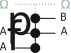
\includegraphics[width=2.5cm]{graphics/development/edit_to_hivent_operations/CRE_to_SEC+UNI}
  } \\

  &
  $n_f$ &
  $n_p$ &
  $1$ &
  \pbox{6.0cm}{
    ~\\
    \texttt{SEC} of $B_1$ from $\Omega$ \\
    \texttt{SEC} of $T_p$ from $A_p$, \texttt{INC} of $T_p$ into $B_1$ \\
    \texttt{INC} of $A_f$ into $B_1$
  } &
  \\

  %%% MERGE %%

  \midrule
  \multirow{3}{*}{\texttt{MRG} (1)} &
  \multicolumn{4}{p{10cm}}{
    Multiple Areas $A_i$ are unified to $B_1$. The new Area receives a name distinct from all the names of $A_i$.
  } &
  \multirow{3}{*}{
    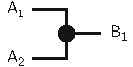
\includegraphics[width=2.5cm]{graphics/development/edit_to_hivent_operations/MRG_to_UNI}
  } \\
  &
  $n \geq 2$ &
  $0$ &
  $1$ &
  \pbox{6.0cm}{
    \texttt{UNI} of $\forall A_i$ to $B_1$
  } &
  \\

  \midrule
  \multirow{4}{*}{\texttt{MRG} (2)} &
  \multicolumn{4}{p{10cm}}{
    Multiple Areas $A_i$ are unified. The resulting Area reuses the short and formal name of one of the old Areas ($A_0$) and therefore preserves it. The remaining Areas $A_i$ are incorporated into $A_0$.
  } &
  \multirow{4}{*}{
    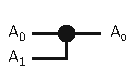
\includegraphics[width=2.5cm]{graphics/development/edit_to_hivent_operations/MRG_to_INC}
  } \\
  &
  $n \geq 1$ &
  $1$ &
  $1$ &
  \pbox{6.0cm}{
    \texttt{INC} of $\forall A_i$ into $A_0$
  } &
  \\

  \midrule
  \multirow{4}{*}{\texttt{MRG} (3)} &
  \multicolumn{4}{p{10cm}}{
    The same as the previous case, just that $A_0$ receives a new short name and therefore an additional name change is required.
  } &
  \multirow{4}{*}{
    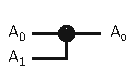
\includegraphics[width=2.5cm]{graphics/development/edit_to_hivent_operations/MRG_to_INC+NCH}
  } \\
  &
  $n \geq 1$ &
  $1$ &
  $1$ &
  \pbox{6.0cm}{
    ~\\
    \texttt{INC} of $\forall A_i$ into $A_0$ \\
    \texttt{NCH} of $A_0$
  } &
  \\

  %%% DISSOLVE %%

  \midrule
  \multirow{4}{*}{\texttt{DIS} (1)} &
  \multicolumn{4}{p{10cm}}{
    Multiple Areas $B_i$ are separated from one initial Area $A_0$. Each $B_i$ receives a part of the territory of $A_0$ and a name. Each name is distinct from the name of $A_0$.
  } &
  \multirow{4}{*}{
    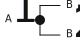
\includegraphics[width=2.5cm]{graphics/development/edit_to_hivent_operations/DIS_to_SEP}
  } \\
  &
  $1$ &
  $0$ &
  $n \geq 1$ &
  \pbox{6.0cm}{
    ~\\
    \texttt{SEP} of $A_1$ into $\forall B_i$
  } &
  \\

  \midrule
  \multirow{5}{*}{\texttt{DIS} (2)} &
  \multicolumn{4}{p{10cm}}{
    Multiple Areas $B_i$ are separated from one initial Area $A_0$. Each $B_i$ receives a part of the territory of $A_0$ and a name. One of the separated Areas has the same short and formal name as $A_0$, so it preserves its identity. The remaining new Areas secede from $A_0$.
  } &
  \multirow{5}{*}{
    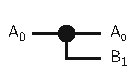
\includegraphics[width=2.5cm]{graphics/development/edit_to_hivent_operations/DIS_to_SEC}
  } \\
  &
  $1$ &
  $1$ &
  $n \geq 1$ &
  \pbox{6.0cm}{
    ~\\
    \texttt{SEC} of $\forall B_i$ from $A_0$
  } &
  \\

  \midrule
  \multirow{4}{*}{\texttt{DIS} (3)} &
  \multicolumn{4}{p{10cm}}{
    The same as the previous case, just that $A_0$ receives a new short name and therefore an additional name change is required.
  } &
  \multirow{4}{*}{
    
\includegraphics[width=2.5cm]{graphics/development/edit_to_hivent_operations/DIS_to_SEC+NCH}
  } \\
  &
  $1$ &
  $1$ &
  $n \geq 1$ &
  \pbox{6.0cm}{
    ~\\
    \texttt{SEC} of $\forall B_i$ from $A_0$  \\
    \texttt{NCH} of $A_p$
  } &
  \\

  %%% CHANGE BORDER %%%

  \midrule
  \multirow{10}{*}{\texttt{CHB} (1)} &
  \multicolumn{4}{p{10cm}}{
    One existing Area $A_0$ is selected and its territory changes. Relative to the old territory some parts of the territory expands ($T_e$) and some withdraws ($T_w$).
    The part of $T_e$ that expands into unclaimed land ($T_\Omega: T_\Omega \in T_e$) is seceded from $\Omega$ and incorporated into $A_0$.
    The Areas $A_f$ fully covered by $T_e$ are incorporated into $A_0$,
    the Areas $A_p$ partially covered by $T_e$ secede this territory $T_p \in T_e$ to $A_0$.
    $T_w$ is be incorporated into $\Omega$, resulting in unclaimed land.
  } &
  \multirow{10}{*}{
    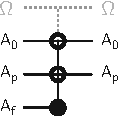
\includegraphics[width=2.5cm]{graphics/development/edit_to_hivent_operations/CHB_to_SEC+INC_omega}
  } \\
  &
  $n_f$ &
  $1+n_p$ &
  $0$ &
  \pbox{6.0cm}{
    ~\\
    \texttt{SEC} of $T_\Omega$ from $\Omega$,
    \texttt{INC} of $T_\Omega$ into $A_0$ \\
    \texttt{SEC} of $T_p$ from $A_p$,
    \texttt{INC} of $T_p$ into $B_1$ \\
    \texttt{INC} of $A_f$ into $B_1$ \\
    \texttt{SEC} of $T_w$ from $B_1$,
    \texttt{INC} of $T_w$ into $\Omega$
  } &
  \\

  \midrule
  \multirow{7}{*}{\texttt{CHB} (2)} &
  \multicolumn{4}{p{10cm}}{
    Two existing Areas $A_1$ and $A_2$ are selected and their common border changes. This results in a symmetrical change of territories, made up by two sets of territories: $T_2$ that previously belonged to $A_1$ and is now part of $A_2$ and $T_1$ for which the opposite is true. $T_2$ is seceded by $A_1$ and incorporated into $A_2$, the opposite happenes to $T_1$.
  } &
  \multirow{7}{*}{
    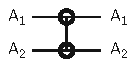
\includegraphics[width=2.5cm]{graphics/development/edit_to_hivent_operations/CHB_to_SEC+INC}
  } \\
  &
  $0$ &
  $2$ &
  $0$ &
  \pbox{6.0cm}{
    ~\\
    \texttt{SEC} of $T_2$ from $A_1$,
    \texttt{INC} of $T_2$ into $A_2$ \\
    \texttt{SEC} of $T_1$ from $A_2$,
    \texttt{INC} of $T_1$ into $A_1$
  } &
  \\

  %%% RENAME %%%

  \midrule
  \multirow{3}{*}{\texttt{REN} (1)} &
  \multicolumn{4}{p{10cm}}{
    One Area $A_1$ is selected and both its short and formal name is changed. Therefore, a new Area $B_1$ is created as a direct successor of $A_1$. This is a special case of a unification with only one Area.
  } &
  \multirow{3}{*}{
    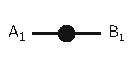
\includegraphics[width=2.5cm]{graphics/development/edit_to_hivent_operations/REN_to_UNI}
  } \\
  &
  $1$ &
  $0$ &
  $1$ &
  \pbox{6.0cm}{
    \texttt{UNI} of $A_1$ to $B_1$
  } &
  \\

  \midrule
  \multirow{3}{*}{\texttt{REN} (2)} &
  \multicolumn{4}{p{10cm}}{
    One Area $A_1$ is selected and receives a new short name, but the formal name and therefore the identity is preserved. $A_1$ is updated.
  } &
  \multirow{3}{*}{
    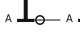
\includegraphics[width=2.5cm]{graphics/development/edit_to_hivent_operations/REN_to_NCH}
  } \\
  &
  $0$ &
  $1$ &
  $0$ &
  \pbox{6.0cm}{
    \texttt{NCH} of $A_1$
  } &
  \\

  %%% CEASE %%%

  \midrule
  \multirow{2}{*}{\texttt{CES} (1)} &
  \multicolumn{4}{p{10cm}}{
    One Area $A_1$ is selected and ceases by incorporating into the universe.
  } &
  \multirow{2}{*}{
    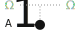
\includegraphics[width=2.5cm]{graphics/development/edit_to_hivent_operations/CES_to_INC}
  } \\
  &
  $1$ &
  $0$ &
  $0$ &
  \pbox{6.0cm}{
    \texttt{INC} of $A_1$ into $\Omega$
  } &
  \\

  \bottomrule
\caption{Translation from Edit Operations to Hivent Operations}
\end{longtable}
\label{tab:editoperations_to_hg_operations}
\end{center}
\footnotetext{multiple Hivent Operations in one row happen exactly at the same time point, so they are combined}


% subsection edit_workflow (end)

% ------------------------------------------------------------------------------
\subsection{Retrospective Updates} % (fold)
\label{sub:retrospective_updates}

A straighforward use case of the Hivent Model is to change the current state of the system with a new Edit Operation into the future. Givent the initial start point $t_0$, a current time point $t_{now} > t_0$ and a set of consecutively added Hivent Operations at $t_i \in [t_0 .. t_{now}[$. The accumulation of all changes make up the current state of the system at $t_{now}$. To change this current state, a new Hivent Operation can be inserted at $t_{now}$ into the future as a \emph{forward operation}. This state is valid until the next change is inserted.

For the purpose of historical research this use case alone is not sufficient, because the current state $t_{now}$ of the map is known to large degree. The problem is to edit states in the past. For this purpose the concept of a \emph{backward operation} comes into play: A Hivent Operation is inserted at time point $t_i$, but into the past: $ t_0 < t_i < t_{now}$. As an example: Given the initial state 10.06.2016 with present-day Germany created on 03.10.1990 on the map. The user wants to enter the German Reunification. The HGIS must support separating Germany into East and West, but indicating that this was the state \emph{before} 1990 and the original state was \emph{after} this date. This is complicated, because the conceptual, data and computational model have to adapt to this requirement.

The Hivent Operations themselves allow to be executed the other way, because each of them has an inverse operation: A \texttt{UNI} can be inverted with a \texttt{SEP} and a \texttt{INC} with a \texttt{SEC} operation. \texttt{NCH} can be inverted with itself by swapping the old and new name.

% - - - - - - - - - - - - - - - - - - - - - - - - - - - - - - - - - - - - - - -
\paragraph{Consistency} % (fold)
\label{par:consistency}

Each Hivent Operation that is not entered as a \emph{forward operation} to the end of the timeline must maintain the semantic, spatial and thematic integrity of the data, i.e. the changes to Areas, their territories and names must still work. All possible conflicts with consecutive Hivent Operations have to be resolved. The simple example in figure \ref{fig:update_conflict_example} shows the problem: Given time point $t_1$ with two Areas $A$ and $B$ and an \texttt{UNI} Hivent Operation at $t_2$ unifying $A$ and $B$ to $C$. If in retrospective a new Hivent Operation is inserted at $t_r: t_1 < t_r < t_2$ that cedes a part of of $A$ to a new Area $X$, the operation at $t_2$ is not consistent anymore, because the old territory of $A$ is not the same. It is not simple to say how the remaining territory $?$ should be treated.

\begin{figure}[H]
  \vspace{1em}
  \centering
  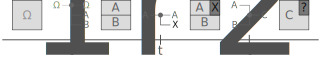
\includegraphics[width=0.8\textwidth]{graphics/development/update_conflict/example}
  \caption{Example for a simple conflict due to a retrospective update}
  \label{fig:update_conflict_example}
\end{figure}

% paragraph consistency (end)

% - - - - - - - - - - - - - - - - - - - - - - - - - - - - - - - - - - - - - - -
\paragraph{Conflicts} % (fold)
\label{par:conflicts}

The way the Hivent Model works is comparable to a version control system like \emph{Git}
\footnote{
  \emph{Git},
  --everything-is-local,
  \url{https://git-scm.com/},
  last access: 29.05.2016
}
Just like in Git, there are different kinds of conflicts that can occur on retrospective updates. In this model, they are classified regarding their resolvability:

\begin{compactenum}
  \item[A)] The conflict can be resolved \emph{\textbf{a}utomatically} without the interference of the user.
  \item[S)] The conflict requires the user to choose between two alternatives (\emph{\textbf{s}emi-automatic} resolution).
  \item[M)] The conflict is complex and the user needs to resolve it \emph{\textbf{m}anually}.
\end{compactenum}

The remaining part of this section examines all possible cases of conflicts and their resolveability. Each inserted Hivent Operation transforms a set of old Areas $A = [A_i]$ to a set of new Areas $B = [B_i]$ or updates an update Area $A_0$ or both. Each consecutive Hivent Operation that manipulates $A_0, A_i \in A$ or $B_i \in B$ has to be checked regarding three aspects of integrity:

\begin{compactenum}
  \item semantic: Does $A_0$ and $\forall A_i \in A$ still exist? If not, can it easily be replaced by another Area?
  \item spatial: Is the territory of $A_0$ and $\forall A_i \in A$ still the same? If not, can it easily by updated?
  \item thematic: Is the name of $A_0$ and $\forall A_i \in A$ still the same? If not, can it easily be updated?
\end{compactenum}

All cases can be broken down to the following scenario. Given an initial state at $t_1$ with three spatial entities on the map ($A_1, A_2, A_3$) and an Hivent Operation at $t_2$ manipulating this set of Areas with one of the five possible operations. This is operation is consistent and is called the original Hivent Operation ($H_o$). Now, a retrospective update $H_r$ with one of the five Hivent Operations manipulating the same set of Areas is inserted at $t_r: t_1 < t_r < t_2$. What happens regarding the semantic, spatial and thematic integrity of $H_o$? There are 25 possible cases, because there are 5 different $H_o$ and five different $H_r$ operations.

% paragraph conflicts (end)

% - - - - - - - - - - - - - - - - - - - - - - - - - - - - - - - - - - - - - - -
\paragraph{Retrospective Unification} % (fold)
\label{par:retrospective_unification}
\texttt{UNI}

% paragraph retrospective_unification (end)

% - - - - - - - - - - - - - - - - - - - - - - - - - - - - - - - - - - - - - - -
\paragraph{Retrospective Separation} % (fold)
\label{par:retrospective_separation}
\texttt{SEP}

% paragraph retrospective_separation (end)

% - - - - - - - - - - - - - - - - - - - - - - - - - - - - - - - - - - - - - - -
\paragraph{Retrospective Incorporation} % (fold)
\label{par:retrospective_incorporation}
\texttt{INC}

% paragraph retrospective_incorporation (end)

% - - - - - - - - - - - - - - - - - - - - - - - - - - - - - - - - - - - - - - -
\paragraph{Retrospective Secession} % (fold)
\label{par:retrospective_secession}
\texttt{SEC}

% paragraph retrospective_secession (end)

% - - - - - - - - - - - - - - - - - - - - - - - - - - - - - - - - - - - - - - -
\paragraph{Retrospective Name Change} % (fold)
\label{par:retrospective_name_change}
\texttt{NCH}

trallala und hoppsassa

% paragraph retrospective_name_change (end)

\vspace{1em}
The final result is visualized in the $5 \times 5$ matrix in figure \ref{tab:conflicts_retrospective_updates}.

\begin{table}[ht]
\begin{center}
\begin{tabular}{p{0.1cm} p{0.1cm} p{0.3cm} cx{2.0cm} cx{2.0cm} cx{2.0cm} cx{2.0cm} cx{2.0cm} cx{2.0cm}}
  \toprule
  & & & & \multicolumn{5}{c}{original Hivent Operation $H_o$} \\
  & & & & \texttt{UNI} & \texttt{SEP} & \texttt{INC} & \texttt{SEC} & \texttt{NCH} \\
  \midrule
    \multirow{5}{*}{\rot{retrospective}}
  & \multirow{5}{*}{\rot{operation $H_r$}}
    & & \texttt{UNI} & A & \textbf{M} & A & A & A \\
  & & & \texttt{SEP} & S(A$|$A) & S(A$|$A) & \textbf{M} & S(A$|$\textbf{M}) & A \\
  & & & \texttt{INC} & A & \textbf{M} & A & A & X \\
  & & & \texttt{SEC} & S(A$|$A) & S(A$|$A) & S(A$|$A) & S(A$|$A) & X \\
  & & & \texttt{NCH} & A & A & X & X & A \\
  \bottomrule
\end{tabular}
\caption{All possible conflicts on retrospective updates regarding their resolvability}
\small{X = no conflict, A = automatic, S = semi-automatic, \textbf{M} = manual resolution \\[-0.1em]
For semi-automatic resolution, the resolveability of the two options is stated like S(\nth{1}$|$\nth{2})}
\label{tab:conflicts_retrospective_updates}
\end{center}
\end{table}

% - - - - - - - - - - - - - - - - - - - - - - - - - - - - - - - - - - - - - - -
\paragraph{Error correction} % (fold)
\label{par:error_correction}

Correcting wrong information in an event-based system is important to understand: Given time point $t_y$ and an Area $A$ with the name $X$. If $X$ happens to be wrong, it means that the historical change at time point $t_x: t_x < t_y$ that created the name $X$ into Area $A$ is erroneous and has be corrected. Correcting a state means correcting the event that created this state.

% subsection retrospective_updates (end)

% section editing_hivent_data (end)